

%\section{How to control a detector?}

\subsection{What is EPICS?} 
\label{EPICS}
EPICS is a set of tools and applications which provide a software infrastructure for distributed control systems \cite{EPICS_license}. This framework could be used for large systems like particle accelerators, telescopes, etc. as well as for smaller systems featuring only several hundred process variables \cite{EPICS_1, EPICS_2, EPICS_3, EPICS_4}.
\begin{figure}[!h]
\centering
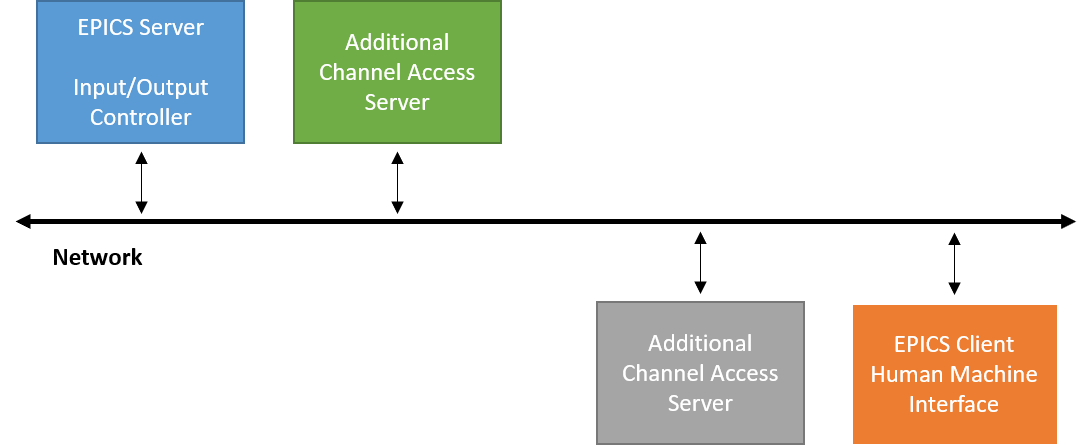
\includegraphics[width=0.7\columnwidth]{Chapter3/Controls/images/EPICS.png}
\caption{EPICS working principle}
\label{fig_EPICS}
\end{figure}
As described in Figure \ref{fig_EPICS}, the system uses client/server and publish/subscribe approaches to communicate between different devices/nodes. Most servers, called Input/Output Controllers ( \gls{IOC}) perform I/O and local control tasks and publish this information to clients via dedicated protocols Channel Access and/or pvAccess \cite{EPICS}. 

 \subsection{Available control tool sets}
 EPICS and related toolkits offer a complete set of applications to control large experiments. Many different sites all over the world have implemented EPICS-based control systems, i.e. \gls{J-PARC} \cite{J-PARC}, \gls{STAR} \cite{STAR}, \gls{ITER} \cite{ITER}, Australian Synchrotron and many more \cite{EPICS_site}. Besides, there are also different alternatives to implementing a control system, which include: 
 \begin{itemize}
     \item Siemens WinCC \cite{Camacho:2022fxa,Goralczyk:2022udx}
     \item Tango \cite{Santander-Vela:2021tma}
     \item Labview \cite{State:2022qlw} 
     \item custom software (e.g. python/C++ or stream processing software) \cite{taurus}
 \end{itemize} 
 These frameworks were discarded either because of licensing needs (Labview, Siemens WinCC) or lack of extensive experience on-site (Tango). Phoebus \cite{Phoebus} was chosen as the collection of tools and applications to monitor and operate \gls{STS}. All \gls{mSTS}'s \glspl{OPI} were prepared in Phoebus \cite{Phoebus}. The detector uses the following Phoebus-related applications:
\begin{itemize}
    \item Alarms logging
    \item Alarm server
    \item Save and restore
\end{itemize}
More details about these applications and their use will be provided in the next sections. Although Phoebus proved to be easy to use and implement new operator screens, there are also alternatives that could provide similar functionalities:
\begin{itemize}
    \item Bluesky Project (Python-based set of libraries \cite{Bluesky}),
    \item React Automation Studio \cite{React},
    \item Channel Access Tools - MEDM, \gls{ALH}, \gls{AR} etc. 
\end{itemize}

\subsection{EPICS architecture and IOC}
The core elements of the systems are the \glspl{IOC}, which provides control logic for the connected hardware. The \gls{IOC} uses channel access and/or PVAccess to communicate with clients and contains also the following parts\cite{IOC}:
\begin{itemize}
    \item \gls{IOC} database -  a memory resident database containing a set of named records of various types \cite{IOC2},
    \item record support - set of support routines defining a record,
    \item device support and drivers - serve access to external devices.
    \item monitors and scanners,
    \item sequencer - an optional extension of the \gls{IOC} which is a finite state machine,
\end{itemize}
An \gls{IOC} doesn't need extensive computing resources, that's why it runs also on low-power single-board computers like Raspberry PI or Odroid. 
 \gls{IOC} are also commonly supported by additional modules, device support, libraries, and \glspl{API} which altogether provide an efficient way to control various devices.
To communicate with devices, an \gls{IOC} uses so-called device support. The most commonly used ones include:
\begin{itemize}
    \item StreamDevice is a generic EPICS device support for devices with a "byte stream" based communication interface. That means devices that can be controlled by sending and receiving strings (in the broadest sense, including non-printable characters and even null-bytes). Examples of this type of communication interface are serial line (RS-232, RS-485, ...), IEEE-488 (also known as GPIB or HP-IB), and telnet-like TCP/IP \cite{StreamDevice},
    \item devModbus \cite{modbus} - includes support for three Modbus standards (TCP, RTU, ASCII), used for control of climatic chambers in the \gls{STS} group,
    \item asynDriver \cite{asyn} - asynchronous driver support, which is an interface that implements a device-specific code to low-level communication drivers. Together with the StreamDevice it's the most commonly used one in the \gls{mSTS}. 
\end{itemize}

In order to ease the deployment process and have a flexible solution for different architectures, images for the \gls{IOC} as well as other \gls{DCS} building blocks were created. These images can be seen as files with code that upon execution result in the initialization of a container. More detailed information about containerization is included in the next chapter. 
 
